Seven technical chapters have culminated to the main event, the numerical experiments and their results. This is where we learn if BNNs can deliver on the promise of substituting direct calculations of cross sections. We will begin with a description of the dataset and the data transformations made prior to training and their potential implications for the predictive performance of the trained BNNs. We will then explain the methodology employed including the implementation details, the selection of BNN models and hyperparameters and performance metrics. Once discussed, we will explore the results and their consequences.


\section{Training Procedure and Selection of Models and Hyperparameters}
For convenience, we repeat the training procedure discussed at the end of chapter \ref{chap:bnn} below.
\begin{enumerate}
    \item The weights of the neural network model is initiated from a the prior, i.e.
    \begin{equation}
        \text{Draw} \quad W^\ell \sim p(W^\ell) \qq{and} \text{draw} \quad b^\ell \sim p(b^\ell) \qq{for} \ell = 1, 2, \ldots, L.
    \end{equation}
    \item A set of pretraining steps are performed using the backpropagation algorithm which is combined by the forward pass in algorithm \ref{algo:forward_pass} and the backward pass in algorithm \ref{algo:backward_pass}. The loss function $\mathcal{L}$, which is the same as the potential energy function used with HMC and NUTS from eq.~\eqref{eq:special_potential_energy}, is minimized using the ADAM optimizer with respect to the network weights to obtain a point estimate. The point estimate is used to initiate the Markov chain. The regularization parameters in eq.~\eqref{eq:special_potential_energy} are set as $\sigma = 1$ for the likelihood and $\lambda_W = \lambda_b = 10^{-3}$ for the priors. This was done for every trained model in this chapter.
    \item A finite number of \textit{warm-up} steps are performed, starting from the point estimate. The warm-up steps are divided into 80\% adaptation steps used to adapt the step size $\epsilon$ used with the Leapfrog integrator. At this point, the step size is freezed and the remaining 20\% is used for burn-in or \textit{mixing}. This is a heuristic recommended by the {\tt TensorFlow-Probability} developers.
    \item Once the warm-up steps are completed, we start gathering neural network samples. We have generated 1000 samples for each BNN model. In each case, these are sampled by skipping 10 samples between each stored sample. This is done to reduce the correlation between successive samples. The total number of samples generated after the warm-up steps is thus really 11000 of which only each 11th sample is kept. As we explained in chapter \ref{chap:bnn}, this is done to reduce the memory footprint of the trained model as correlated samples will bias any MCMC estimator computed using eq.~\eqref{eq:mcmc_estimator}.
\end{enumerate}
All models discussed in this chapter are trained using the procedure above.

In order to better understand the behaviour of BNNs, we have chosen to train a set of models whose details are listed in table \ref{tab:deep_models}. Each model consists of 1000 sampled neural networks. Each model is trained with $\tanh(x)$ as the activation function on the hidden layers, while the output layer uses an identity activation. We will refer this table whenever a model or a set of models selected from it is used. Otherwise, we will state the model architecture used and its hyperparameters explicitly. 
\begin{table}[H]
    \centering
    \caption{
        The table shows a selection of models that is used for benchmarking purposes in this chapter. For each model, 1000 sampled networks were sampled to collectively represent each BNN model.
        We performed 1000 pretraining epochs with a batch size of 32 using the ADAM optimizer. We used 2500 warm-up steps (80\% adaptation steps first, followed by 20\% burn-in steps). For every sampled network, we skipped 10 samples. The kernel used for each model was the NUTS kernel with a maximum of $L = 4096$ Leapfrog steps.
        The number of nodes per layer is shown in the ``Layers'' column.
    }
\begin{tabular}{c@{\hspace{1cm}}c@{\hspace{1cm}} c}
\hline
      Model number & Layers & Number of parameters \\
\hline
    1 & 5-50-1 & 351\\
    2 & 5-50-50-1 & 2901\\
    3 & 5-50-50-50-1 & 5451\\
    4 & 5-50-50-50-50-1 & 8001\\
    5 & 5-50-50-50-50-50-1 & 10551\\
\hline
\end{tabular}
\label{tab:deep_models}
\end{table}
 

\section{Results and Discussion}\label{sec:results}
In this section we present the results from various numerical experiments and discuss their implications. We start off with measurement of computational performance with a focus on training time, prediction time and loading times. We then investigate the posterior distribution projected onto two-dimensional planes of the BNN weights to investigate their potential multi-modal nature in order to evaluate if the typical approximations with surrogate distributions for the weights yield a sufficient representation of the exact posterior distribution. Following this, we present the effect various hyperparameters have on the training of BNNs. Finally, we explore the predictive distributions of various trained BNNs.


\subsection{Computational Performance}
In this thesis we are primarily concerned with creation of an optimized alternative to direct calculations of NLO cross sections.
In this section we will explore the computational performance of BNN models, both on modern CPUs and GPUs. We shall measure the training time which, with the way we perform Bayesian inference of the BNN parameters, most appropriately translates to the time used per generated sample with HMC and NUTS. Another measurement of great interest is the time a trained BNN model uses to compute predictions as this will be their central limiting factor once trained. However, because we must store the full BNN model on disk, the loading times play an important role as well. We shall therefore measure the execution time of predictions and loading times separately.
We will perform wall clock measurements using {\tt time.perf\_counter} provided by the {\tt time} module of the standard library shipped with Python 3. It yields a measurement in fractional seconds of the clock with the highest available resolution on the system.

Note that {\tt TensorFlow} supports OpenMP-type parallelization on the CPU. The workload is evenly distributed among the threads (which may be physical cores or virtual threads if the CPU has hyperthreading support). It is a form of shared-memory parallelization in which all threads access the same memory. This is similar to how a GPU operates.
Unfortunately, multi-device parallelization either on the CPU or the GPU lacks support in the case of non-synchronous execution. Thus we will only compare the single-node performance that is achievable with either a CPU or a GPU. We will thus contrast the performance achieved by a single CPU node with several (virtual) threads available to the performence obtained by employing the workloads on the GPU.

\subsubsection{CPU v. GPU Training Performance}
On which commercially available hardware platform training should be executed is of great interest from a practical standpoint as 
sampling from neural network posteriors is notoriously expensive due to the high-dimensional parameter space its weights reside in.
In this section we pit the training performance achieved on a CPU and GPU against each other.

In figure \ref{fig:relative_performance}, we demonstrate the significant speedup that can be achieved
with GPU accelerated sampling when using {\tt TensorFlow-Probability} and its implementation of samplers. Here we have used HMC and a fixed $L = 512$ Leapfrog steps with XLA (Accelerated Linear Algebra) compilation enabled on the GPU. This is a highly optimized linear algebra execution engine that can significantly speed up code written with {\tt TensorFlow} run on an NVIDIA GPU \cite{xla}. The models trained had the architechture 5-$n$-1 with various choices of number of hidden layer nodes $n$.
By inspection we see that for the model with the largest number of parameters, the GPU can achieve approximately 50 times speedup relative to the CPU.
From the figure at the bottom, we can note that the corresponding absolute wall clock time per generated sample on the GPU took roughly 0.5 seconds. We performed 1000 warm-up steps and sampled 1000 neural networks skipping 10 between each stored sample. Thus in practice, we generated 12000 neural networks in total (1000 for the warm-up steps and 11000 during sampling) which each on average took 0.5 seconds. This amounts to a total time of roughly 1.67 hours. To generate the same number on the CPU, then, would require a total wall clock time of approximately 83.5 hours. Thus training BNNs on a GPU can yield a significant practical benefit, especially as the complexity of the model increases. 

In the same manner we did with the analysis here, one can estimate the total training time of the BNNs by performing a test run to generate a fair number of samples from which the wall clock time per sample can be estimated. The analysis is is slightly more convoluted when the NUTS sampler is used instead. Since the NUTS sampler adaptively sets the number of Leapfrog steps, only an upper-bound on the wall clock time can be estimated by measuring the wall clock time used with HMC in the following manner. When using NUTS, a maximum tree depth $J$ is set which corresponds to a maximum number of Leapfrog steps $L = 2^J$. Measuring the wall clock time with HMC, fixing the number of Leapfrog steps to $L = 2^J$ will yield an upper-bound on the wall clock time used by NUTS. The estimated time will likely be larger than what the NUTS sampler actually uses as it may terminate the tree doubling before reaching the maximum tree depth. This approach is sensible as the computational cost of the NUTS sampler is approximately the same as for HMC for an equivalent number of Leapfrog steps when using a sufficiently complex model and/or a large dataset, as we discussed in chapter \ref{chap:no_u_turn_sampler}.

\begin{figure}[H]
    \centering
    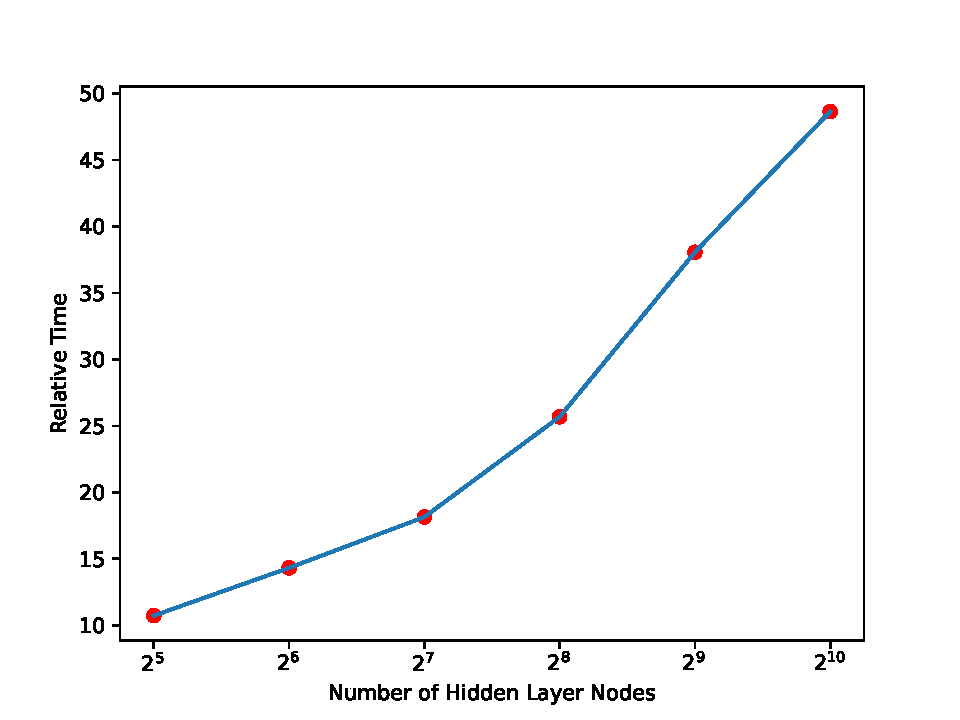
\includegraphics[scale=0.7]{figures/cpu_vs_gpu/cpu_vs_gpu_performance.pdf}
    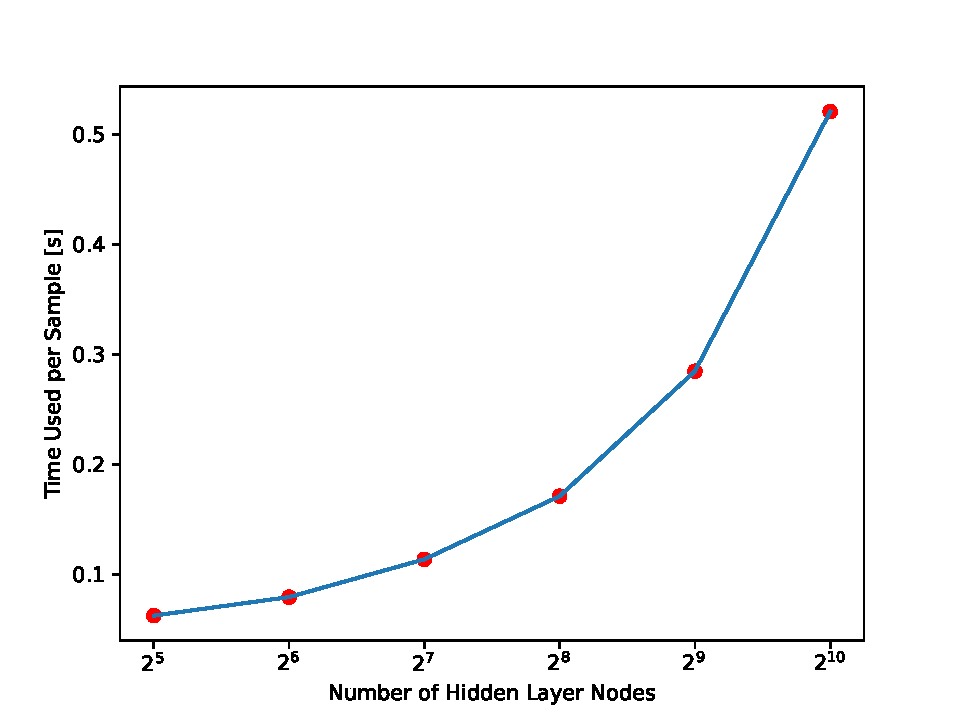
\includegraphics[scale=0.7]{figures/cpu_vs_gpu/gpu_training_time.pdf}
    \caption{The figure on top shows the relative wall clock time used per generated sample using $L = 512$ Leapfrog steps with the HMC sampler,
    as a function of number of hidden nodes in the hidden layer with an architechture 5-$n$-1, where $n$ represents the number of nodes. The relative wall clock time is computed as the wall clock time used by the CPU divided by the wall clock time used by the GPU. The figure on the bottom shows the absolute wall clock time per generated sample measured on the GPU for the same case. The red dots indicate the actual measured points. The CPU measurements are done using an 8-core M1 CPU (Apple Silicon). The GPU measurements
    are made on an NVIDIA Tesla P100 GPU.
    }
    \label{fig:relative_performance}
\end{figure}

\subsubsection{Prediction Time}
As we discussed in chapter \ref{chap:physics_problem}, the execution time's order of magnitude when using {\tt Prospino} can be up to the order of hours. 
If BNNs are to serve as a viable alternative to these calculations, it must at least significantly reduce the time it takes to compute predictions. In figure \ref{fig:prediction_time}, we 
show the average execution time to compute predictions using the models in table~\ref{tab:deep_models}.
For each model, we randomly generated input points $x\in \mathbb{R}^5$ and computed predictions for up to 4096 input points simultaneously.
Thus the largest input for the BNNs were of dimension $(4096, 5)$. The execution times were measured in 1000 trials from which the sample mean were computed.
The execution times appear proportional to the number of input points provided for each model, which perhaps is not all that surprising. We can crudely infer by inspection that increasing the order of magnitude by one does the same for the execution time. Still, the order of magnitude for a single input point is at the order of a millisecond which is a significant speedup over {\tt Prospino} calculations. Both the sample mean of the predictions and the sample error were computed during the measurement. 

\begin{figure}[H]
    \centering
    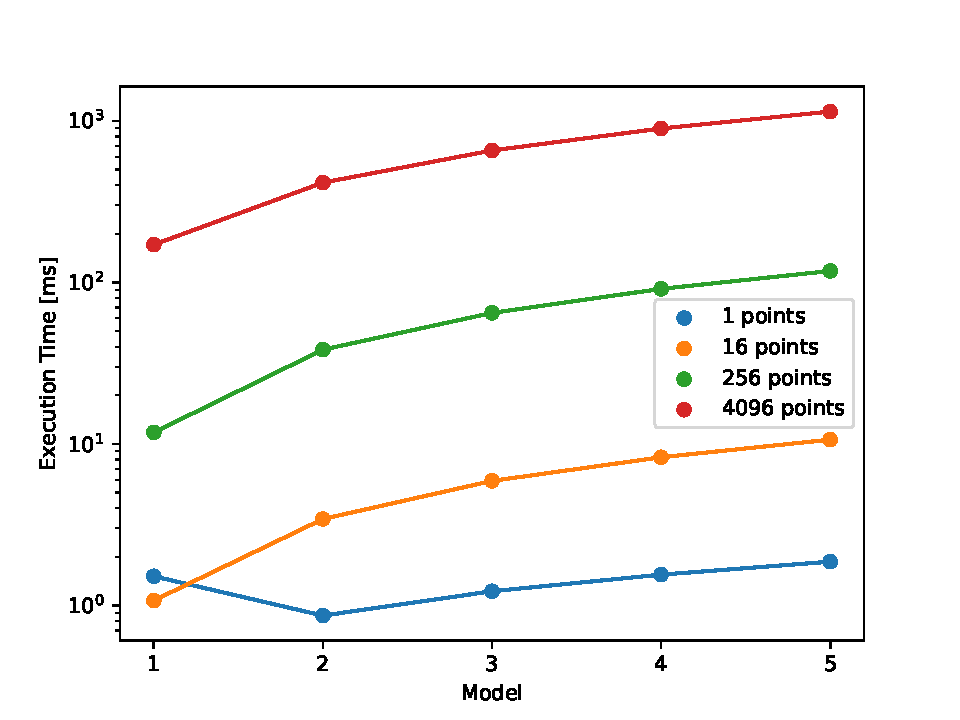
\includegraphics[scale=0.7]{figures/prediction_time/prediction_time.pdf}
    \caption{The figure shows the average prediction time given up to several simultaneous inputs $x$ using the models in table \ref{tab:deep_models}. The wall clock time of the executions shown are measured in milliseconds and are averaged over 1000 trials per case. The measured wall clock time includes computation of the sample mean and sample error of the predictive distribution produced by the BNN models. The dots indicate the actual measured values. The colored graphs indicate how many simultaneous input points that were used. The measurements were done using an 8-core M1 CPU (Apple Silicon).
    }
    \label{fig:prediction_time}
\end{figure}

The performance degradation observed in figure \ref{fig:prediction_time} that occur as we increase the number of simultaneous input points is inherently due to the limited vectorization capability of the CPU's computing units when performing matrix multiplications in the forward pass of the individual neural network models. The computation itself is performed with all 1000 sampled networks simultaneously, and so one might hypothesize that more specialized computing units may be able to handle several input points while applying all sampled networks at the same time. As it turns out, GPUs excel at executing matrix multiplication. In figure \ref{fig:prediction_time_gpu} we can see the execution times achieved using the GPU on an M1 Apple Silicon SoC to perform the same computations as before. In this case the order of magnitude remains more or less the same in all the tests. Thus, computing predictions on several simultaneous input points can be of a great benefit if the execution is employed on a GPU. Note, however, that the measured execution time of ``model 1'' for a single point is slightly slower than for more points which likely is due to the overhead introduced by using the GPU for such a simple model. Care should thus be taken when considering what type of hardware the computations should be performed with.


\begin{figure}[H]
    \centering
    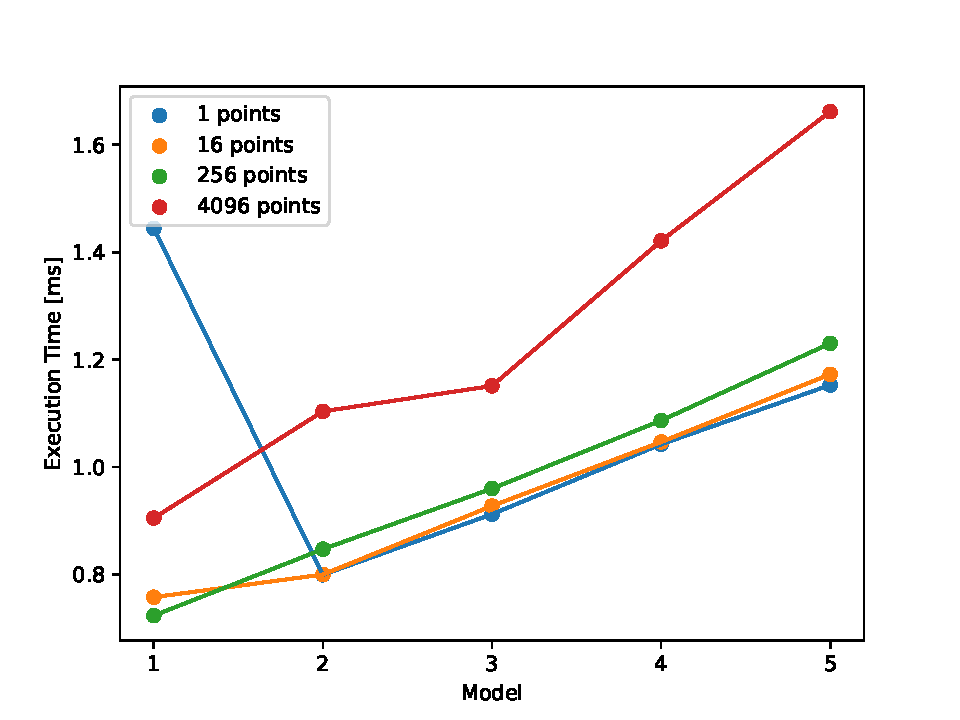
\includegraphics[scale=0.7]{figures/prediction_time/prediction_time_gpu.pdf}
    \caption{The figure shows the average prediction time using the built-in GPU on an M1 Apple Silicon system-on-chip to compute a prediction given a up to several simultaneous inputs $x$ using the models in table \ref{tab:deep_models}. The measured wall clock time is given in milliseconds and is averaged over 1000 trials. The measured time includes computation of the sample mean and sample error of the predictive distribution produced by the BNN models. The dots indicate the actual measured values. The colored graphs indicate the number of simultaneous input points used in each case.
    }
    \label{fig:prediction_time_gpu}
\end{figure}

\subsubsection{Loading Times}
Even if we have demonstrated a substantial speedup for the execution part of computing predictions using BNNs, we have thus far ignored the fact that the empirical distribution representing the weights of the BNN is stored on disk which typically means a solid state drive (SSD) with modern computing hardware. The memory bandwidth between the SSD and the faster forms of memory such as RAM, cache and registers can be a potential bottleneck for performance. Although cache and registers introduce fast memory transfer of stored data to the computing units of the CPU, they typically boast a very limited capacity. Thus loading in the entire BNN model might not be viable and we may observe that once we need models with a large number of parameters, the loading times dominate the computational cost involved with computing predictions. This added computional cost stems from the transfer of data back and forth between the RAM, and the cache and registers. An additional problem is that if the BNN model is simply used for a single prediction at a time, it might simply be loaded a single time before it is dumped from working memory. In this case, the initial load may dominate the computational cost all together. 

In figure \ref{fig:loading_times} we show the resulted loading times (wall clock, as usual) measured using an M1 Apple Silicon system-on-chip. The memory allocated to the BNN models was deallocated manually using the {\tt del} operator provided by Python to ensure that each model was dumped from cache/registers between each measurement. The models loaded in are the ones listed in table \ref{tab:deep_models}. The order of magnitude of the loading times displayed in the figure is approximately the same order of magnitude as the execution time. Thus loading does not seem to display a performance bottleneck for the models used. In other words, we have demonstrated that BNNs can provide a serious substitute for {\tt Prospino} calculations from a purely computational perspective. It remains to be seen if the predictions themselves are reliable enough for this substitution to be adopted, which we will explore in later sections.

\begin{figure}[H]
    \centering
    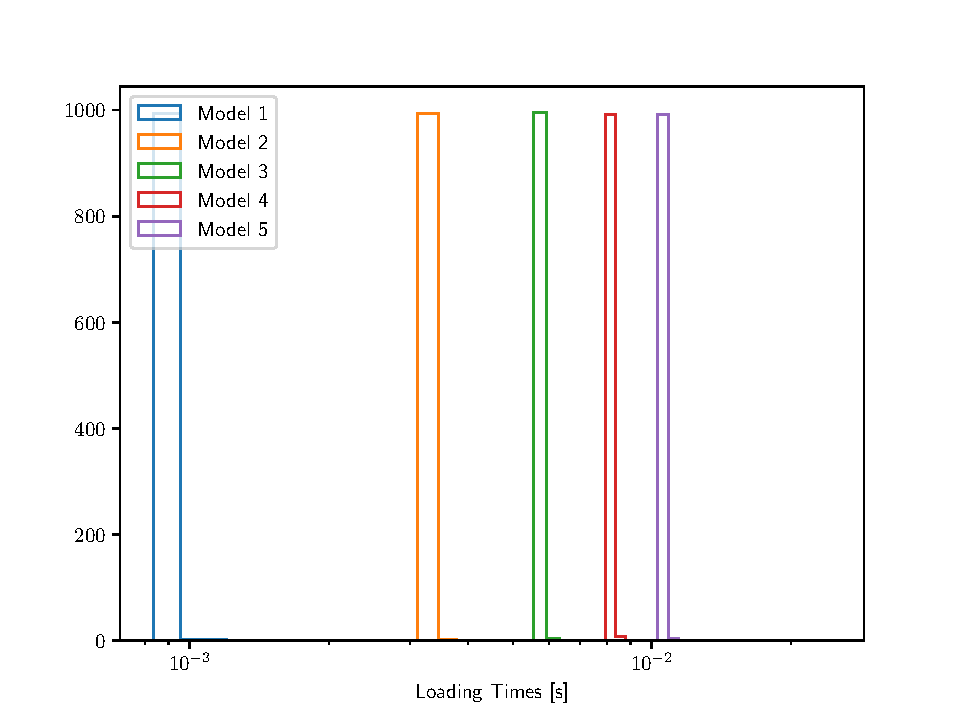
\includegraphics[scale=0.7]{figures/computational_cost/loading_times.pdf}
    \caption{
        The figure shows the histograms of measured loading times (wall clock) in seconds using the models in table \ref{tab:deep_models}. The measurements were made on an M1 Apple Silicon system-on-chip. The time measurements consist of 1000 measurements for each model.
    }
    \label{fig:loading_times}
\end{figure}



\subsection{Posterior Distribution of Weights}
An important problem to consider is if we can even justify the use of Monte Carlo samplers to sample from the exact posterior instead of using the approximation employed by variational inference with a parameterized surrogate posterior, which is the most ubiquitous method of training BNNs in the literature. The surrogate posterior distribution is usually a factorized Gaussian distribution of the form
\begin{equation}\label{eq:surrogate_dist}
    p \propto \prod_{i, j, \ell} \mathcal{N}(\mu_{ij}^\ell, (\sigma_{ij}^\ell)^2) \mathcal{N}(\mu_{j}^\ell, (\sigma_{j}^\ell)^2),
\end{equation}
meaning for each parameter in the model, we assume its posterior distribution can be written as an independent Gaussian distribution with a mean $\mu_{jk}^\ell$ and a standard deviation $\sigma_{ij}^\ell$ for the kernels, and $\mu_j^\ell$ and $\sigma_j^\ell$ for the biases. The method sports some fairly obvious advantages like the fact that one can perform \textit{online training}, i.e. continue training once new data becomes available starting from an earlier \textit{checkpoint} by using $p$ obtained during earlier training as the prior. The way we have trained BNNs in this thesis does not permit this form of training because we cannot formulate a prior based on the empirical distribution we have sampled. Once could perhaps perform kernel density estimation of the empirical distribution to obtain a log-prior which can be used as part of the potential energy function in $\mathcal{L}$. There are, however, a number of practical issues that arise from this idea. The high-dimensional nature of the neural network model class would suggest that a fairly high number of samples relative to the dimensionality of the sample space must be generated to approximate the posterior well. A possibility is to perform kernel density estimation to obtain an approximate density $\hat{\pi}(W, b)$ which an be used during the evaluation of the potential energy function by replacing the priors typically used with $\hat{\pi}(W, b)$. However, the weights of the BNN models are not in general independent of each other and thus kernel density estimation must be performed on the entire sample space which in general will introduce a computational cost that is likely to be intractible.
In practice, then, we cannot use the weights of the model that we have already sampled to continue training. We must start over entirely and discard the empirical distribution we obtained with the prior dataset since the new posterior distribution will change when new data becomes available. If the new data is sufficiently different from the training data used before, the empirical distribution will likely not approximate the posterior very well and keeping them will introduce a bias to MCMC estimators when combined with samples from the new exact posterior.

It has been widely discussed that BNN posteriors are typically found to be multi-modal \cite{google_bnn_posteriors}. We demonstrate this observation in figure \ref{fig:posterior_weights}. 
\begin{figure}[H]
    \centering
    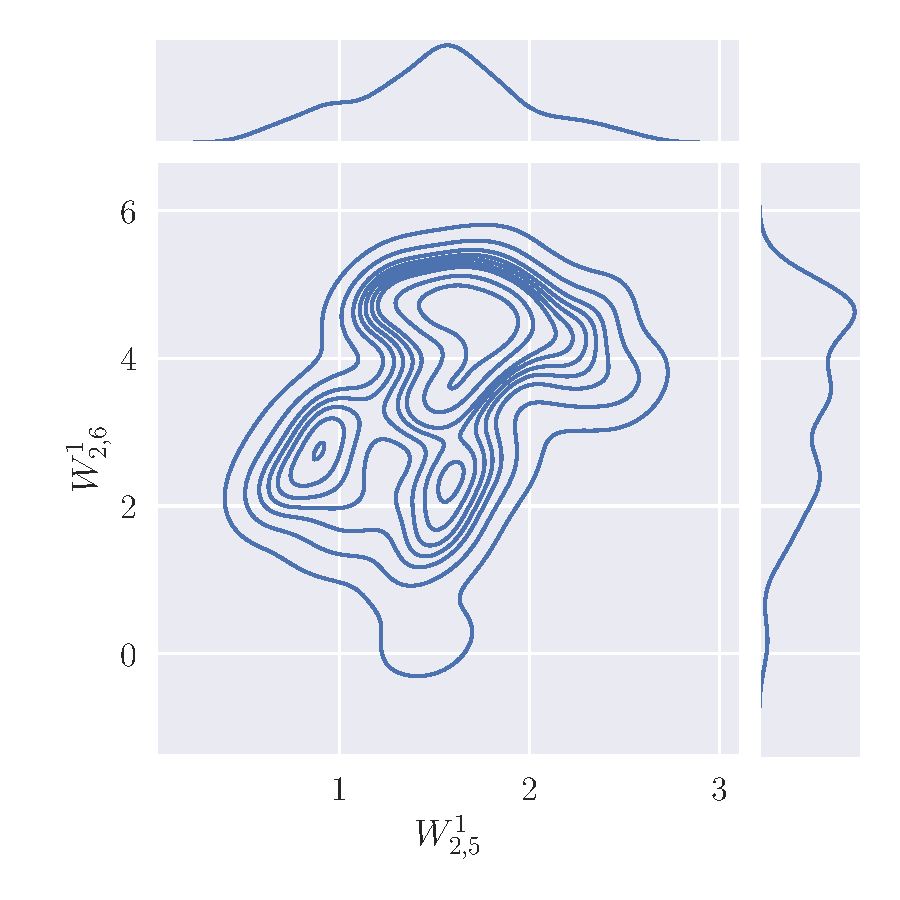
\includegraphics[scale=0.4]{figures/posterior_distribution/posterior_weights_0.pdf}
    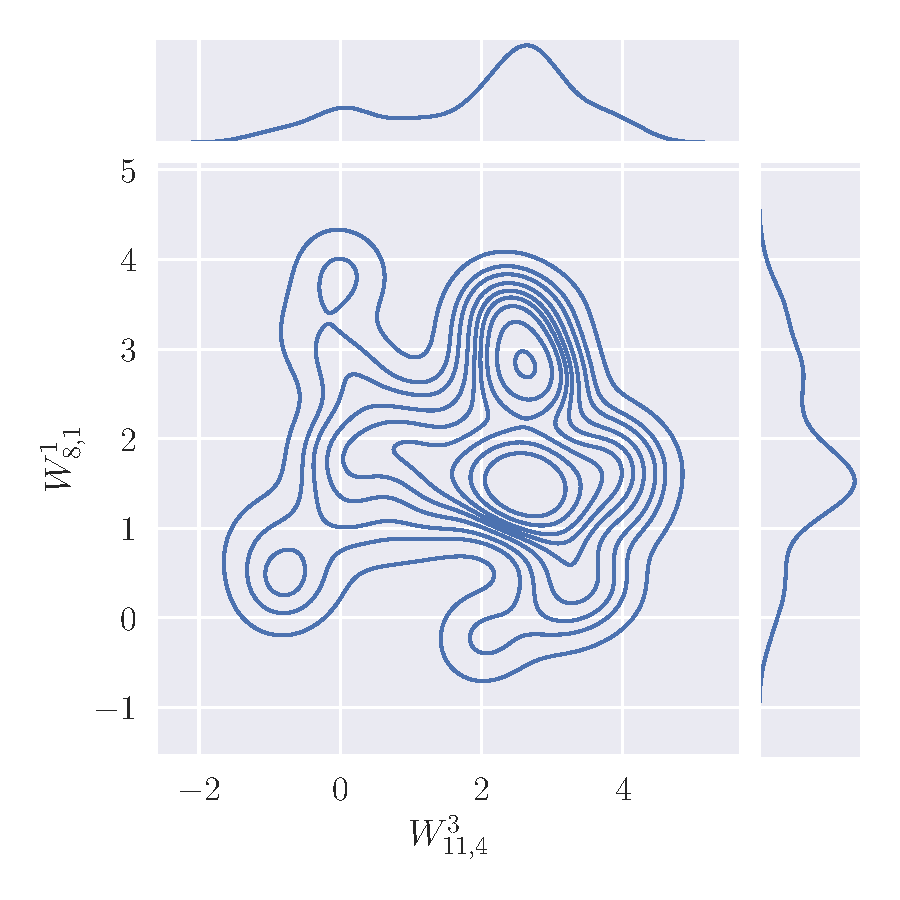
\includegraphics[scale=0.4]{figures/posterior_distribution/posterior_weights_1.pdf}
    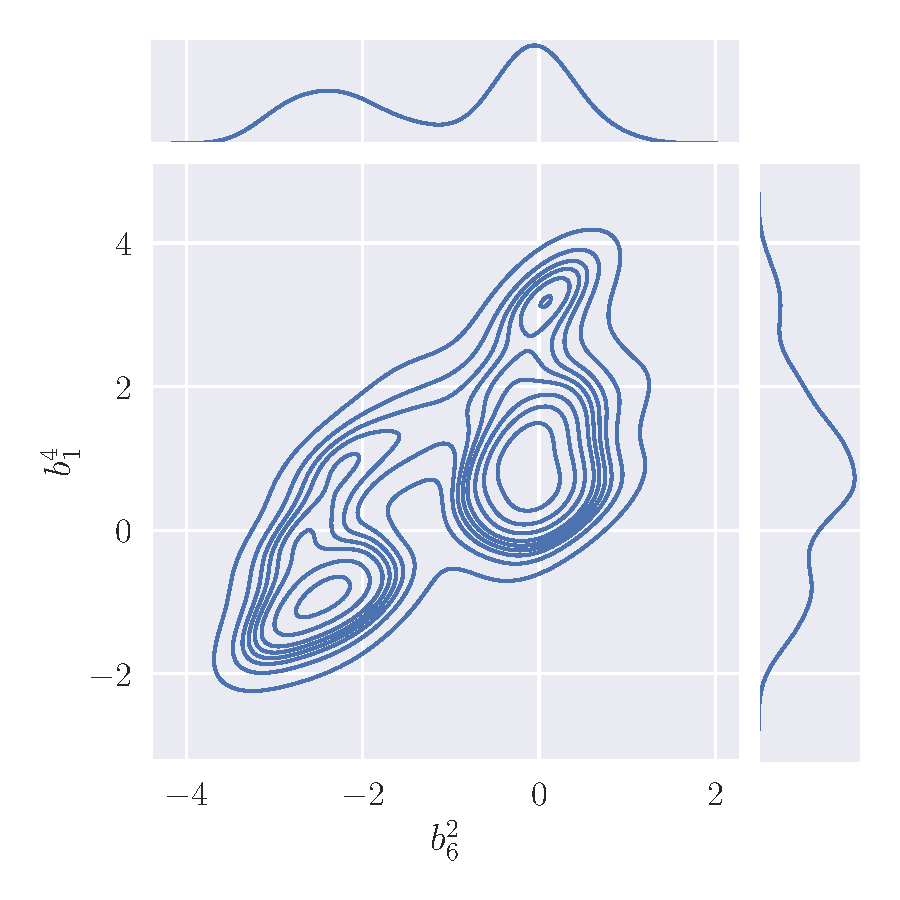
\includegraphics[scale=0.4]{figures/posterior_distribution/posterior_weights_2.pdf}
    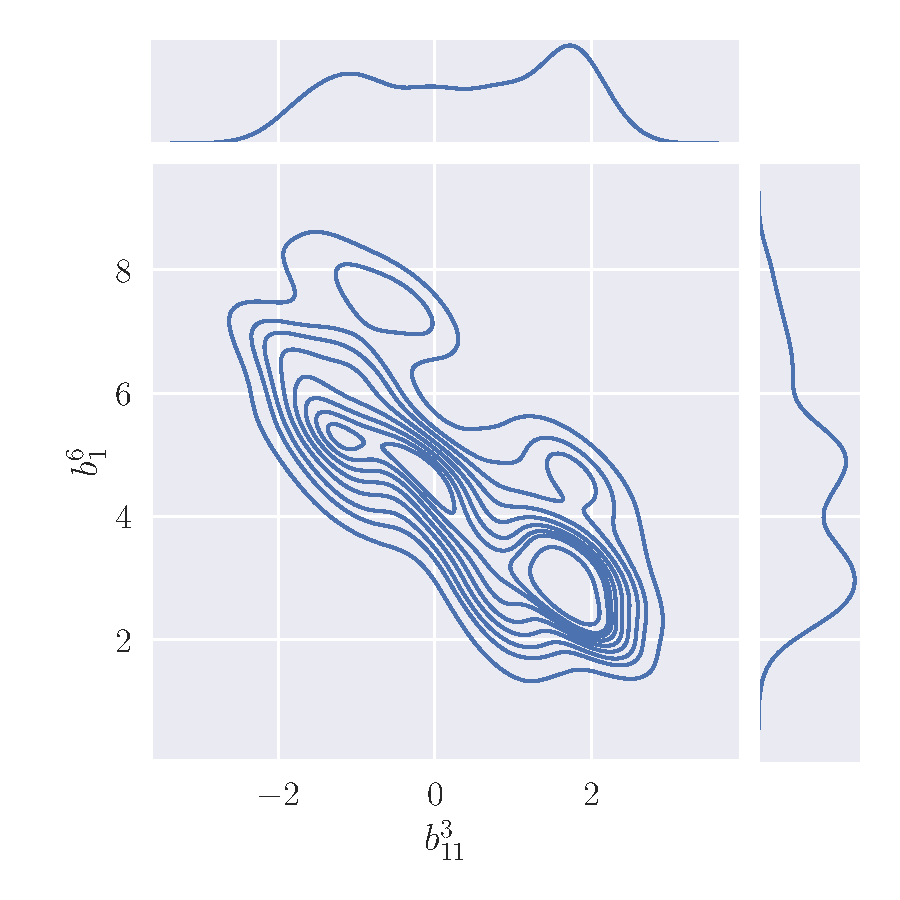
\includegraphics[scale=0.4]{figures/posterior_distribution/posterior_weights_3.pdf}
    \caption{The figure shows the projection of the kernel density estimation of the empirical distribution onto two-dimensional subplanes of the posterior distribution. The figure on the top left shows the plane spanned by $(W_{2,5}^1, W_{2,6}^1)$. The figure on the top right shows the distribution in the plane spanned by $(W_{11,4}^3, W_{8,1}^1)$. The figure on the bottom left shows the distribution in the plane spanned by $(b_6^2, b_1^4)$. The figure on the bottom right shows the distribution spanned by the plane $(b_{11}^3, b_1^6)$. The weights used are the ones pertaining to ``model 4'' in table \ref{tab:deep_models}.
    }
    \label{fig:posterior_weights}
\end{figure}
\noindent It shows the distributions obtained with kernel density estimation applied to projections of the empirical distribution onto two-dimensional planes of the posterior.
We can observe that the projection onto the planes shown there indicate that the posterior distribution indeed is multi-modal
and unlikely to be approximated well with a parameterized surrogate distribution like the one in eq.~\eqref{eq:surrogate_dist}. We cannot make any comments on the specific effect the multi-modality has on the predictive distribution from these results though, only that the distribution itself is poorly approximated by surrogate distributions.



% \begin{figure}[H]
%     \centering
%     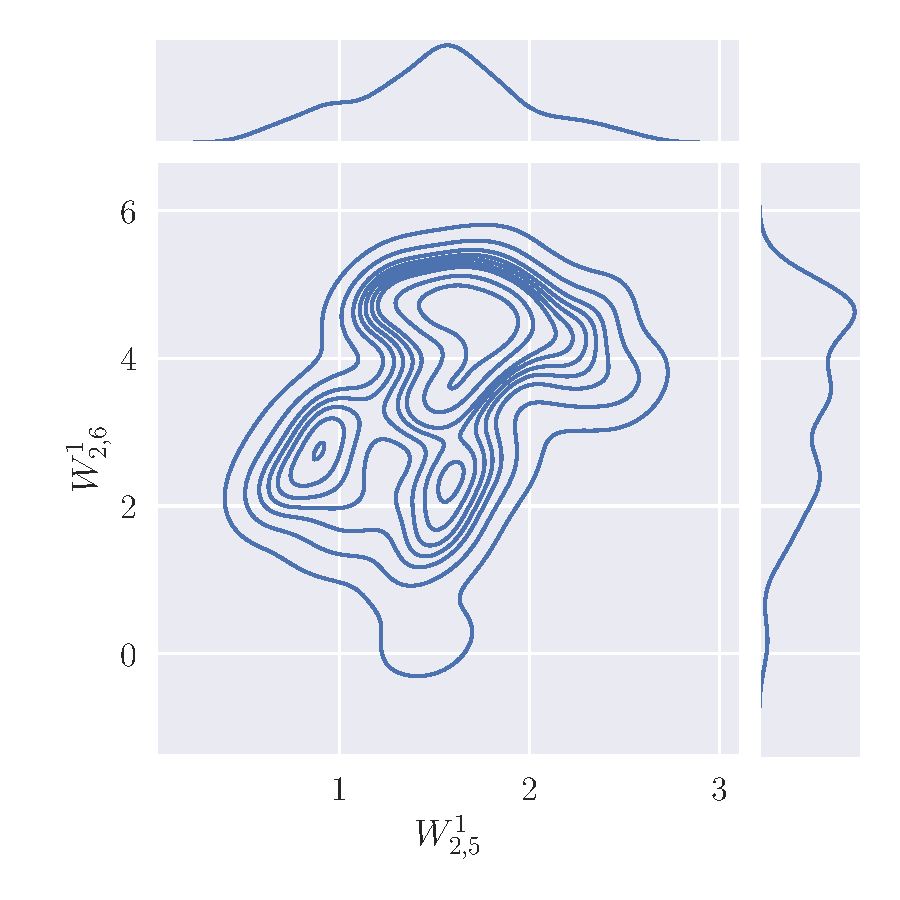
\includegraphics[scale=0.4]{figures/posterior_distribution/posterior_weights_0.pdf}
%     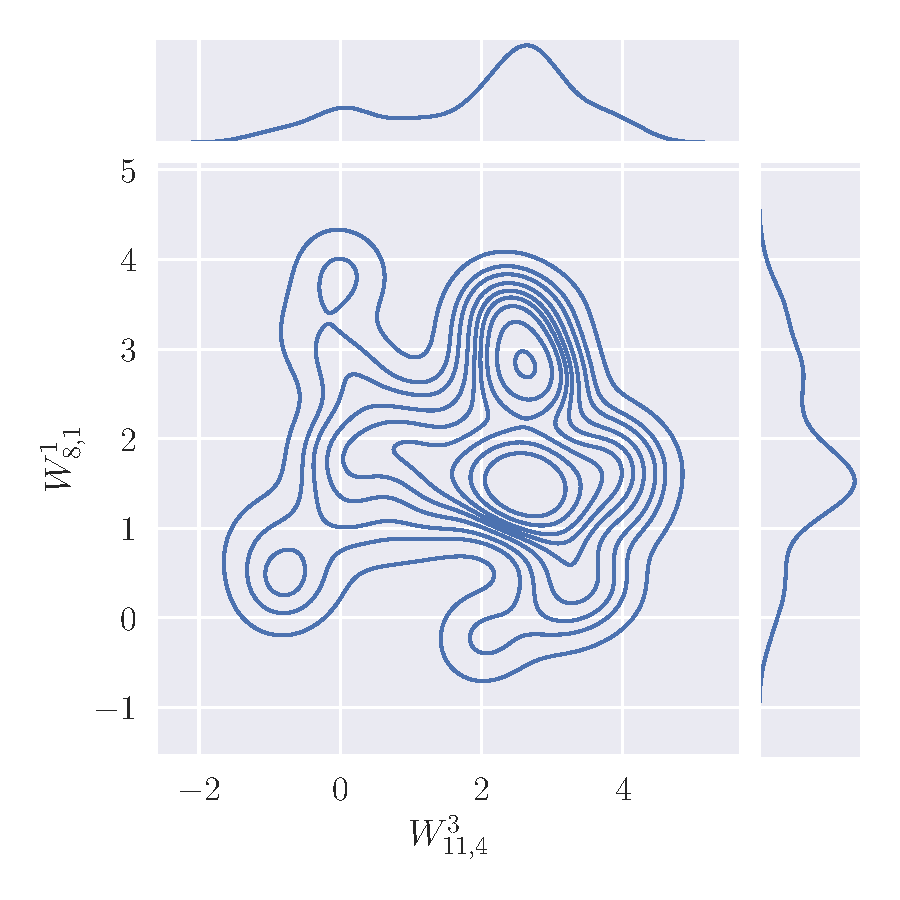
\includegraphics[scale=0.4]{figures/posterior_distribution/posterior_weights_1.pdf}
%     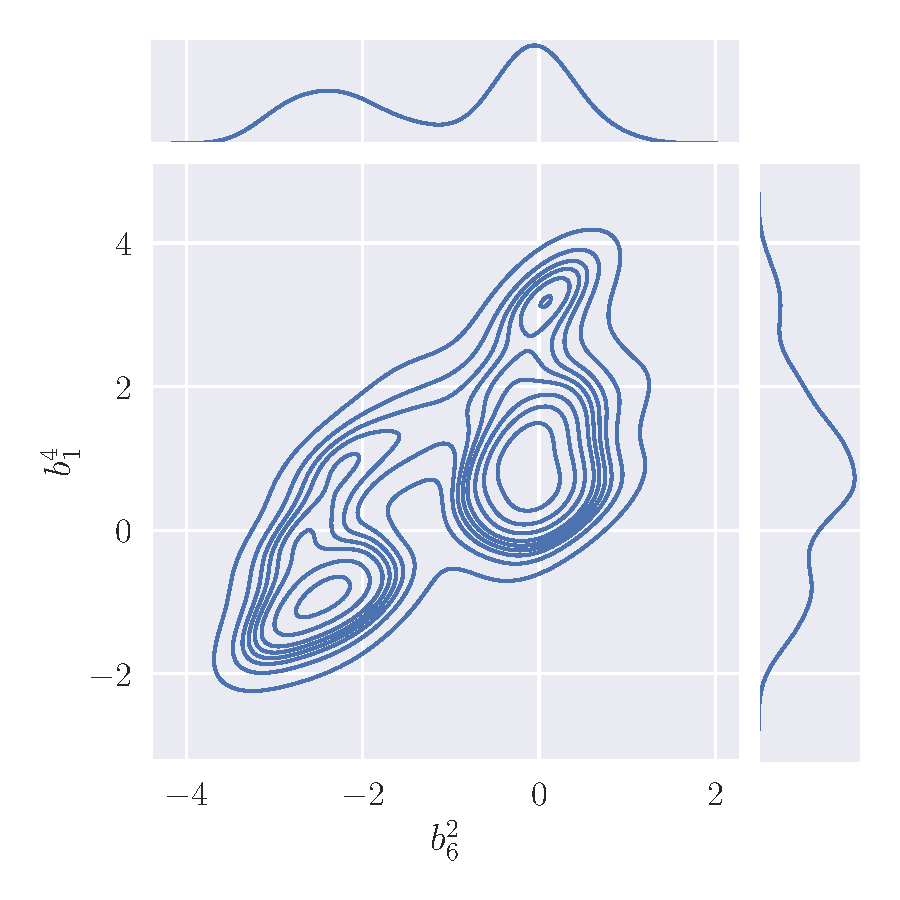
\includegraphics[scale=0.4]{figures/posterior_distribution/posterior_weights_2.pdf}
%     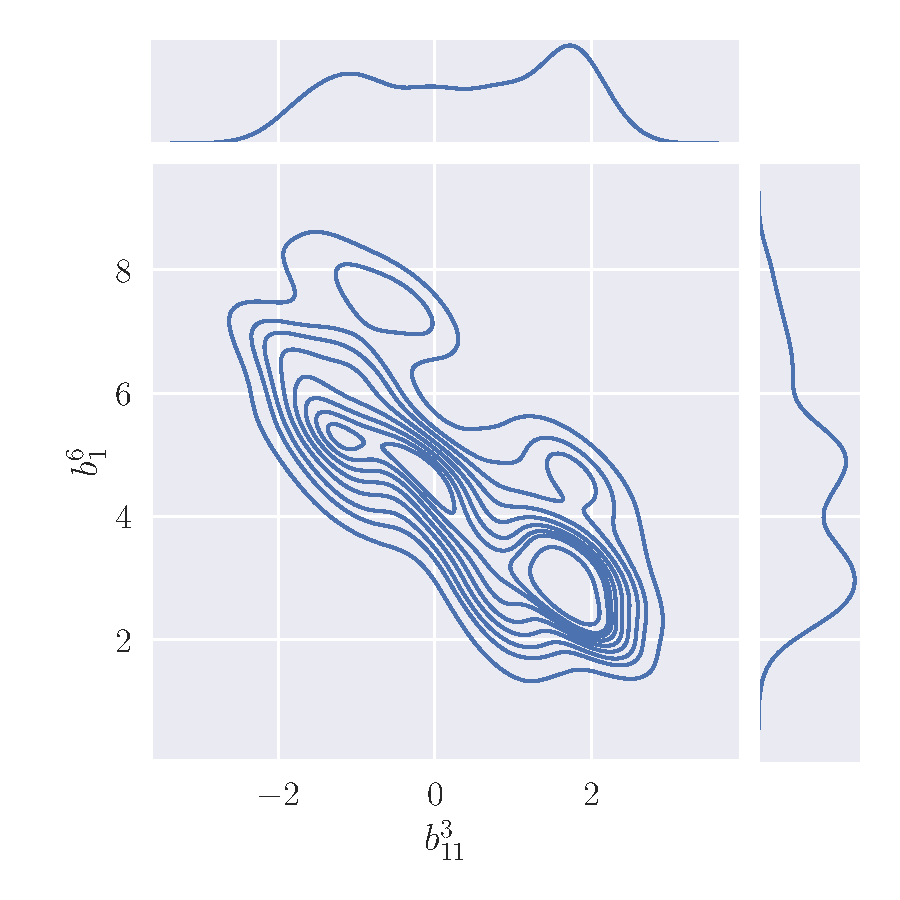
\includegraphics[scale=0.4]{figures/posterior_distribution/posterior_weights_3.pdf}
%     \caption{The figure shows the projection of the empirical distribution onto the planes spanned by $(W_{2,4}^1, W_{2,5}^1)$ on the left and onto the plane spanned by $(W_{3,7}^1, W_{3, 6}^1)$ on the right, using the samples from model 3 in table \ref{tab:deep_models}. The distributions are approximated using kernel density estimation. 
%     }
%     \label{fig:posterior_weights}
% \end{figure}


\subsection{Benchmarks of Hyperparameters}\label{subsec:benchmarks}
In this section, we turn our attention to the effect of various hyperparameters on the performance of the trained BNNs. 
We will investigate the effect of the amount of warm-up and pretraining performed, the effect of increasing the complexity of the models, and how HMC and NUTS affects the performance of the trained models. 

% \begin{figure}[h!]
%     \centering
%     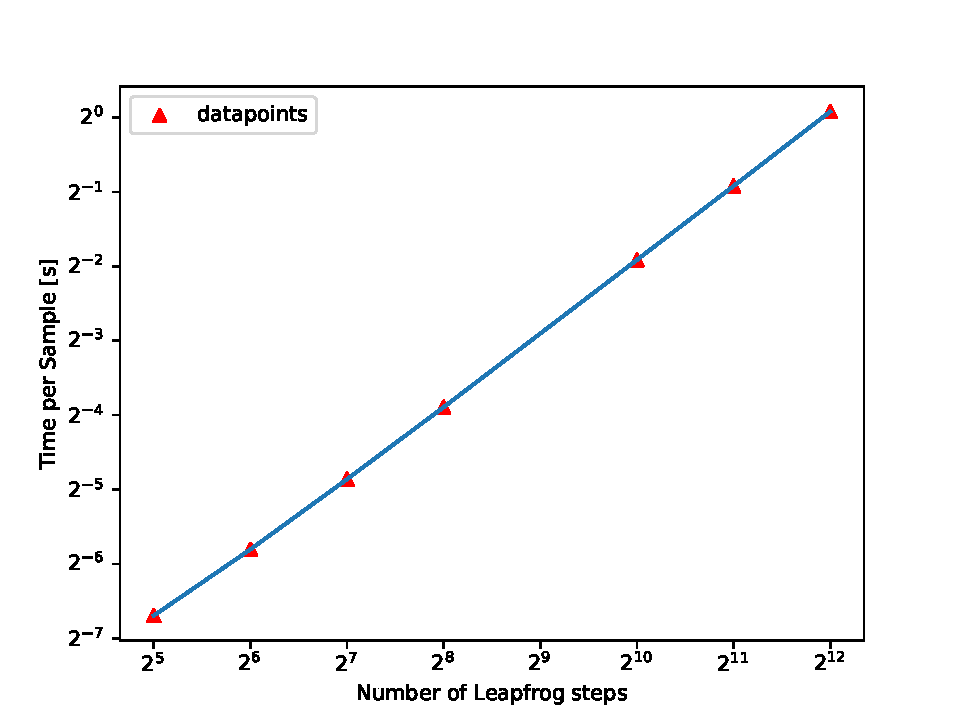
\includegraphics[scale=0.7]{figures/computational_cost/time_vs_leapfrogsteps_hmc.pdf}
%     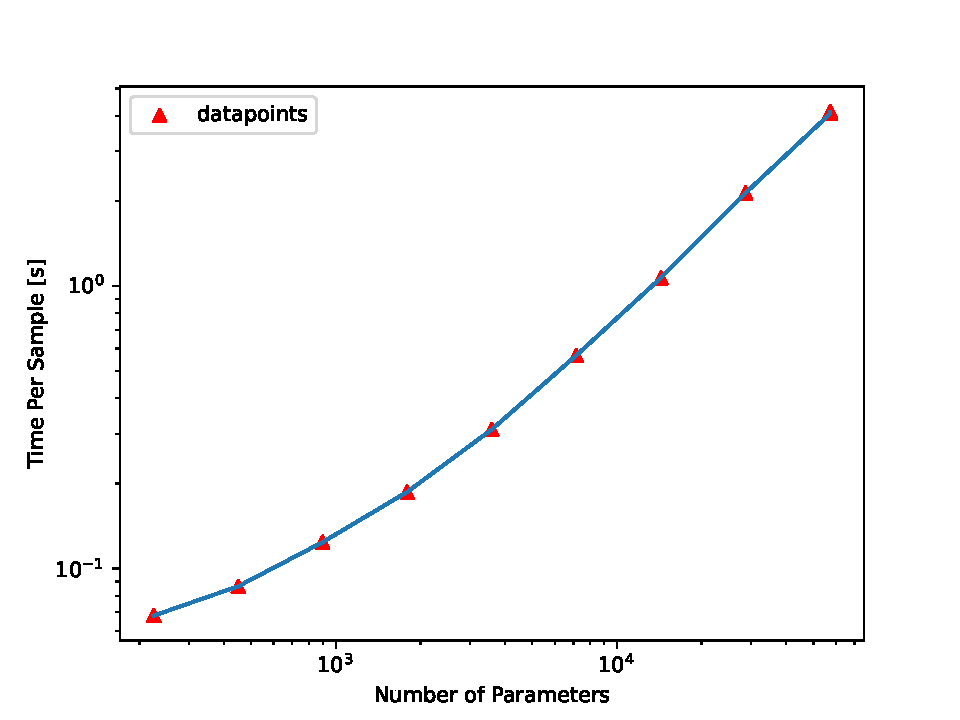
\includegraphics[scale=0.7]{figures/computational_cost/time_vs_params.pdf}
%     \caption{The figure at the top shows the measured time in seconds per sample using HMC as a function of Leapfrog steps $L$ using a model with
%     561 parameters. The figure at the bottom shows the time in seconds per sample with the same sampler with a fixed number of Leapfrog steps $L = 512$ as a function of number of parameters in the BNN model.
%     }
%     \label{fig:time_vs_leapfrogsteps}
% \end{figure}

\subsubsection{The Effect of Number of Warm-up Steps}
As we discussed in section \ref{sec:practical_bnn}, we set a predetermined number of warm-up steps, i.e. number of burn-in steps and number of adaptation steps when using {\tt TensorFlow Probability}'s samplers.
Conventional wisdom would have us believe that increasing the number of burn-in steps increases the probability that the Markov chain has converged
to the stationary distribution of the posterior. Moreover, the literature has shown that NUTS performs at least as good as or better than HMC with an equivalent number of maximum Leapfrog steps or more as the results in \cite{nuts} demonstrated. In our case we have split the number of warm-up steps 80\% adaptation steps which are used to adapt the step size used with the Leapfrog integrator and 20\% burn-in steps to achieve mixing and converge to the stationary distribution. The performance of HMC and NUTS depend heavily on a well-tuned step size, so allocating most of the warm-up steps for this purpose. This will help with efficient exploration of the sample space of the posterior distribution.

To investigate the effect of the number of warm-up steps, we employed a model with a 5-20-20-1 architechture using $\tanh(x)$ as the activation function on the hidden layers. We fixed the number of pretraining epochs to 2500 with a batch size of 32 using the ADAM optimizer.
We then trained several models using various number of warm-up steps with both HMC and NUTS. When trained with HMC, we fixed the number of Leapfrog steps to $L = 512$. When trained with NUTS, we set a maximum tree depth of $12$ corresponding to a maximum of $L = 4096$ Leapfrog steps.
In figure \ref{fig:r2_score_vs_burn_in_steps} we show the achieved $R^2$-scores of the different configurations both in log space and target space as function of the number of warm-up steps used. In log space, the models consistently achieve scores $R^2 \approx 1$ which suggest they on average correctly predict the targets in the test data. Transforming the predictions and targets back to target space, however, lead to som fairly poor results as we increase the number of warm-up steps with HMC outperforming the models trained with NUTS in all but one case. We removed the point at 32 warm-up steps for the NUTS sampler as it achieved a poor score of $R^2 = -1306$ in this case. 
The poor performance in target space is expected if the models in log space do not perform exceptionally well due to the exponentiation of the inverse transform back to target space. Thus we have an empirical confirmation of the potential downside to the data transformations discussed in section \ref{sec:data_transform}.
\begin{figure}[H]
    \centering
    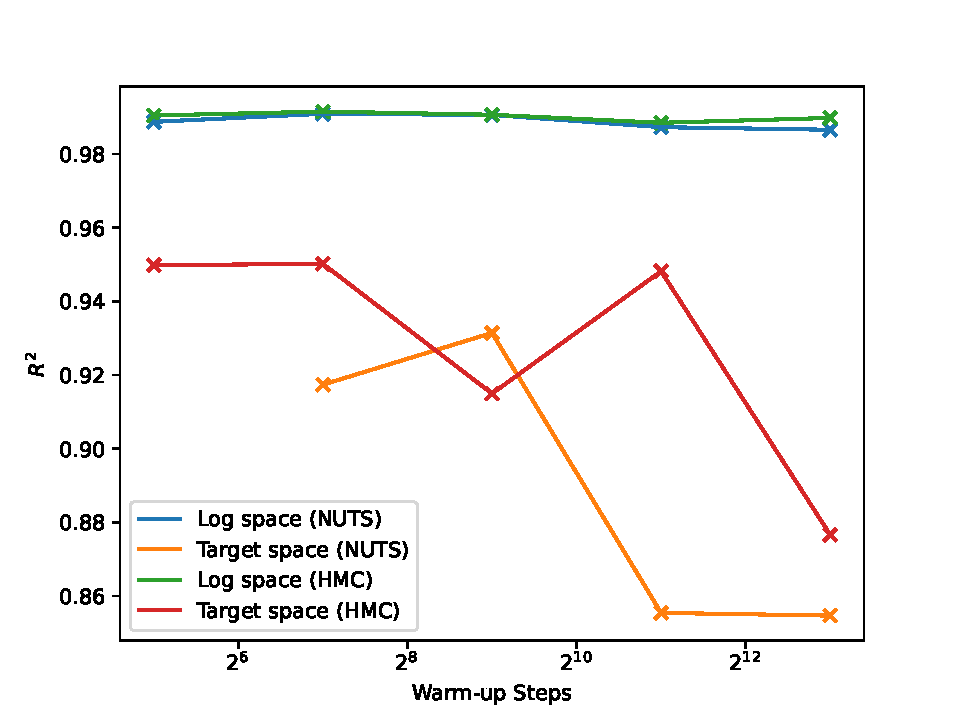
\includegraphics[scale=0.7]{figures/r2_scores/effect_of_burnin_r2_scores.pdf}
    \caption{
        The figure shows the computed $R^2$-scores in both log space and target space as a function number of warm-up steps (20\% burn-in and 80\% adaptation) achieved with HMC and NUTS. The architecture of the BNN model used is 5-20-20-1 with $\tanh(x)$ used as the activation function in the hidden layers. We performed 2500 pretraning steps with a batch size of 32 using the ADAM optimizer. In total 1000 neural networks were sampled with 10 steps between each stored sample. When HMC was used, we ran with a fixed number of Leapfrog steps $L = 512$. When the NUTS sampler was used, we allowed for a maximum of $L = 4096$ Leapfrog steps (a maximum tree depth of $12$).
    }
    \label{fig:r2_score_vs_burn_in_steps}
\end{figure}

In figure \ref{fig:standardized_residuals_vs_burn_in_steps} we display the standardized residuals in log space for both samplers over all trained configurations. 
The standardized residuals demonstrate that the claims discussed in the beginning of this section may not be general enough to apply to BNNs as the models trained with HMC performs better than those trained with NUTS almost regardless of how many warm-up steps that are performed. When using NUTS, the performance of the model trained with a substantial amount of warm-up steps appear to degrade as opposed to improve. The standardized residual of HMC lies consistently inside the Normal distribution for the bulk of the distribution albeit with longer tails, while the NUTS sampler produced rather few models that achieve the same. These results, then, actually indicate that we may be better off running the training procedure of BNNs with a fixed $L$, only adapting the step size. Even better, we may get by with a fairly small number of warm-up steps and a fairly small $L$ as the performance does not appear to depend much on the number of warm-up steps. A small number is likely still necessary to tune the step size used with the Leapfrog integrator. 
\begin{figure}[H]
    \centering
    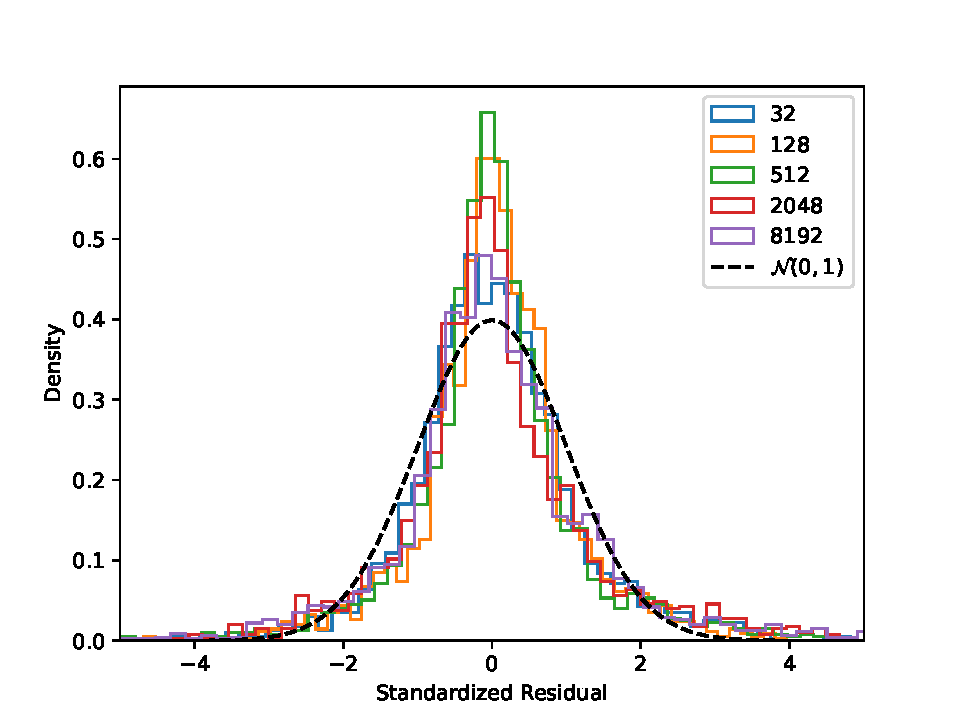
\includegraphics[scale=0.6]{figures/standardized_residuals/effect_of_burnin/standardized_residuals_hmc_vs_burn_in_steps.pdf}
    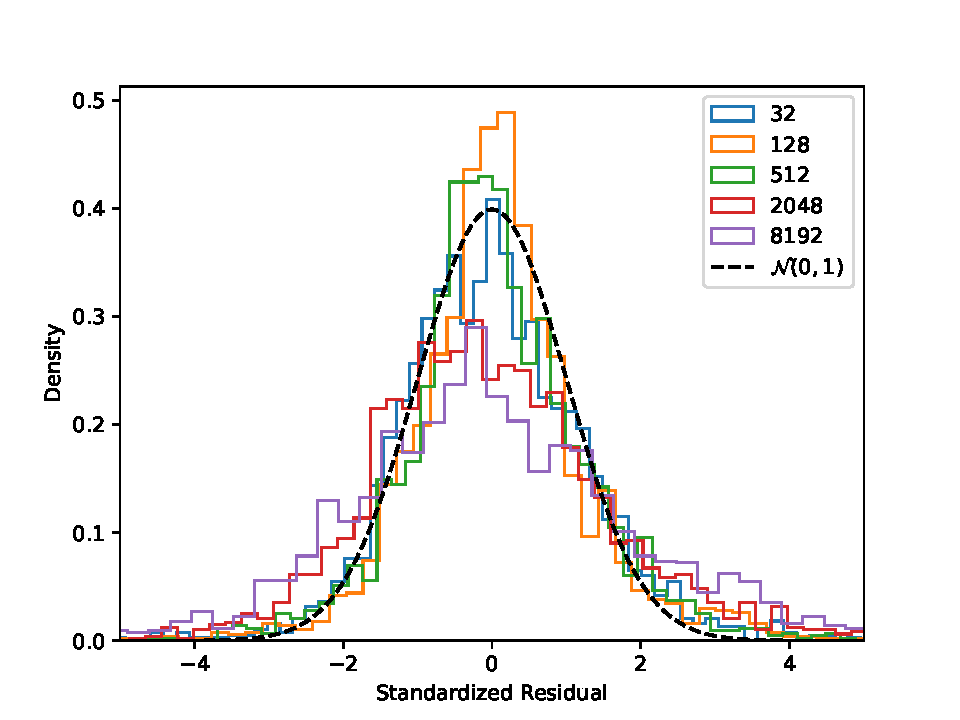
\includegraphics[scale=0.6]{figures/standardized_residuals/effect_of_burnin/standardized_residuals_nuts_vs_burn_in_steps.pdf}
    \caption{The figure shows the standardized residuals computed on the test set. The model architechture used is a model with layers 5-20-20-1 with $\tanh(x)$ as the hidden activation function. In the top figure, we have used the HMC sampler with a fixed number of Leapfrog steps $L = 512$. In the bottom figure, we have used the NUTS sampler with a maximum tree depth of $12$ corresponding to a maximum of $L = 2^{12} = 4096$ Leapfrog steps. The remaining important hyperparameters were 2500 pretraining epochs with a batch size of 32 using the ADAM optimizer. In total 1000 neural networks were sampled in each case with a thinning-amount of 10 steps between each sample. The colors indicate how many warm-up steps that were used. The dotted line is the standard Normal distribution.
    }
    \label{fig:standardized_residuals_vs_burn_in_steps}
\end{figure}


The claim that NUTS performs at least as well as HMC with an equivalent number of Leapfrog steps begs the question, then, how many Leapfrog steps did NUTS use on average? In figure \ref{fig:avg_leapfrog_steps_vs_burn_in}, we show the average number of Leapfrog steps the NUTS sampler used during the generation of the Markov chain as a function of number of warm-up steps. Clearly, NUTS used more Leapfrog steps on average than $L = 512$, except in a single case. The NUTS sampler introduces the need for a slightly more complicated analysis than a one-to-one comparison like this though. Recall from chapter \ref{chap:no_u_turn_sampler}, that the NUTS sampler generates samples by running HMC forwards and backwards in time at random until a stopping condition is met. At this point the sampler selects one of the acceptable states that does not violate detailed balance at random. Thus the selected position (model parameter) may lie close to the initial position.
When trained with HMC, the final state produced by the Leapfrog integrator is accepted with a probability computed according to eq.~\eqref{eq:hmc_acceptance}. Thus the model parameter selected by the HMC sampler at each step is either the initial one or the final one. Thus for the same number of Leapfrog steps and a properly tuned step size, we might expect HMC to generate larger jumps in sample space. The step size used for the two sampler were likely different as the step size adaptation will also differ a bit. The NUTS sampler uses the average acceptance probability for all states generated during the final doubling of the balanced binary tree, while HMC only use the acceptace probability of the final state for step size tuning.

\begin{figure}[H]
    \centering
    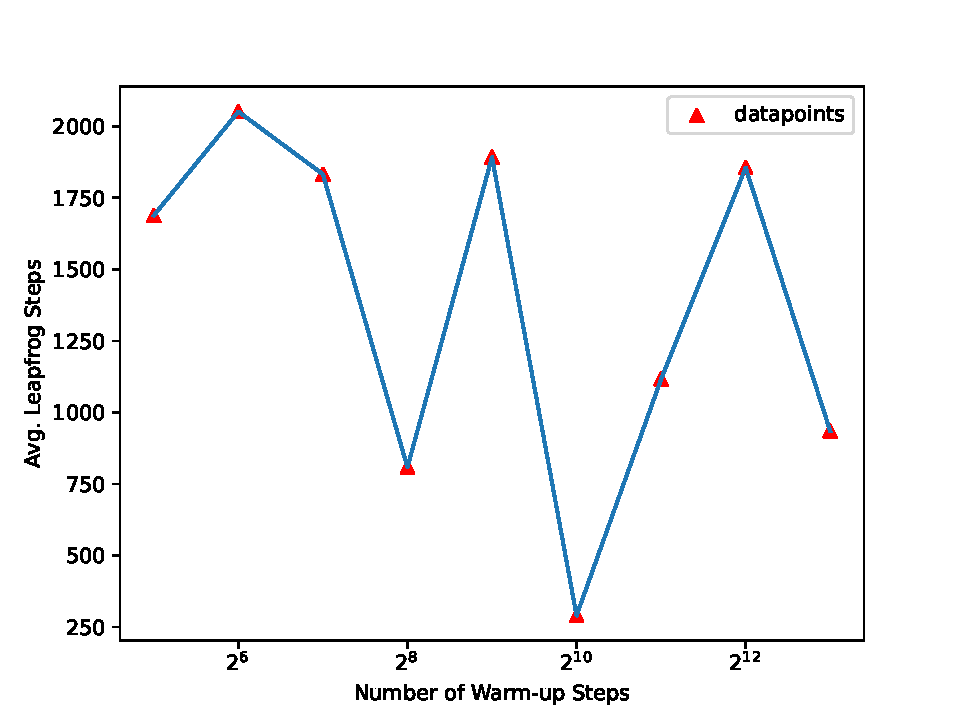
\includegraphics[scale=0.7]{figures/standardized_residuals/effect_of_burnin/avg_burnin_steps_nuts_vs_burn_in_steps.pdf}
    \caption{The figure shows the average number of Leapfrog steps $L$ as a function of number of warm-up steps used by the NUTS sampler when sampling the models shown in the bottom of figure \ref{fig:standardized_residuals_vs_burn_in_steps}. We have included a few more measurements to showcase how fluctuating the average number can be. 
    }
    \label{fig:avg_leapfrog_steps_vs_burn_in}
\end{figure}


\begin{comment}
\begin{table}[h!]
    \centering
    \caption{
        The table shows the computed $R^2$-scores in both log space and target space for an increasing number of warm-up steps (20\% burn-in and 80\% adaptation) achieved with HMC and NUTS. The architecture of the BNN model used is 5-20-20-1 with $\tanh(x)$ used as the activation function in the hidden layers. We performed 2500 pretraning steps with a batch size of 32 using the ADAM optimizer. In total 1000 neural networks were sampled with 10 steps between each stored sample. When HMC was used, we ran with a fixed number of Leapfrog steps $L = 512$. When the NUTS sampler was used, we allowed for a maximum of $L = 4096$ Leapfrog steps (a maximum tree depth of $12$).
    }
\begin{tabular}{c@{\hspace{1cm}}c@{\hspace{1cm}}c@{\hspace{1cm}} c}
\hline
    Sampler & Warm-up steps & $R^2$ (Log space) & $R^2$ (Target space)\\
\hline
    HMC & 32 & 0.990 & 0.950 \\
    HMC & 128 & 0.992 & 0.950 \\
    HMC & 512 & 0.991 & 0.915 \\
    HMC & 2048 & 0.988 & 0.948\\
    HMC & 8192 & 0.990 & 0.877\\
    NUTS & 32 & 0.989 & -1306 \\
    NUTS & 128 & 0.991 & 0.917 \\
    NUTS & 512 & 0.991 & 0.931 \\
    NUTS & 2048 & 0.987 & 0.855 \\
    NUTS & 8192 & 0.987 & 0.855 \\
\hline
\end{tabular}
\label{tab:r2_burn_in}
\end{table}
\end{comment}

% \begin{figure}[h!]
%     \centering
%     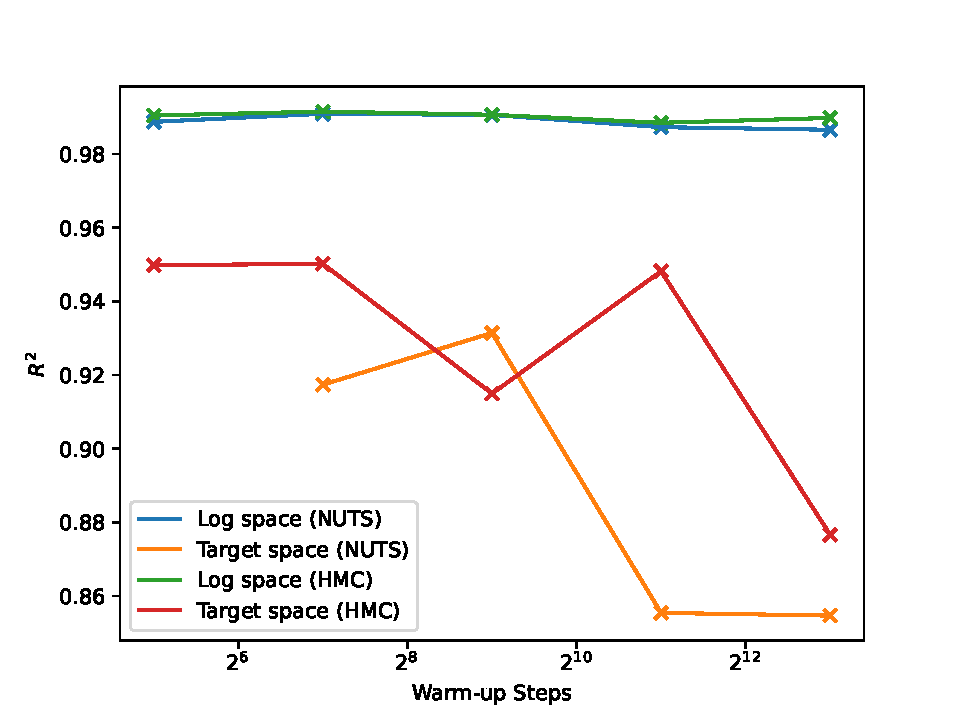
\includegraphics[scale=0.7]{figures/r2_scores/effect_of_burnin_r2_scores.pdf}
%     \caption{
%         The figure shows the computed $R^2$-scores in both log space and target space as a function number of warm-up steps (20\% burn-in and 80\% adaptation) achieved with HMC and NUTS. The architecture of the BNN model used is 5-20-20-1 with $\tanh(x)$ used as the activation function in the hidden layers. We performed 2500 pretraning steps with a batch size of 32 using the ADAM optimizer. In total 1000 neural networks were sampled with 10 steps between each stored sample. When HMC was used, we ran with a fixed number of Leapfrog steps $L = 512$. When the NUTS sampler was used, we allowed for a maximum of $L = 4096$ Leapfrog steps (a maximum tree depth of $12$).
%     }
%     \label{fig:r2_score_vs_burn_in_steps}
% \end{figure}





\subsubsection{The Effect of Pretraining}
Pretraining a BNN model is a strategy employed that starts from a neural network model sampled a random from its prior, and minimizes the potential energy function $\mathcal{L}$ with respect to its weights \textit{before} the Markov chain is initiated to obtain a point estimate that serves as the initial state of the Markov chain. The strategy is suggested as a means to accelerate convergence to the stationary distribution, bypassing the need for long warm-up chains. This may help but as we discussed in chapter \ref{chap:mcmc}, the typical set, the set which we seek to sample from, may not lay particularly close to the mode of the posterior distribution density (recall that minimization of the potential energy function is equivalent to maximizing the posterior distribution density). That said, this systematic search for an initial point for the Markov chain may fair better than initiating it from a randomly drawn sample. Nevertheless, we have a good reason to challenge this recommendation and verify that it indeed improves the performance of the BNN models we sample. Though it should not be surprising if the point estimate yields a better initial point of the Markov chain than one randomly sampled from the priors.

We trained a BNN model with the architechture 5-20-20-1 with $\tanh(x)$ as the activation function in the hidden layers. We fixed the number of warm-up steps to 1000 of which 800 were used for adaptation of the step size and 200 were used for burn-in. We fixed the number of Leapfrog steps to $L = 512$ using the HMC sampler. As usual, we sampled 1000 neural networks with 10 steps between each sampled network. In figure \ref{fig:r2_score_vs_pretraining} we can observe that the performance of the model increases as we increase the number of pretraining epochs which gives us empirical grounds for initiating the Markov chain from the point estimate obtained. As in the previous section, we see a dramatic decrease in performance when we transform the predictions back to target space and compute the $R^2$-score. 
\begin{figure}[H]
    \centering
    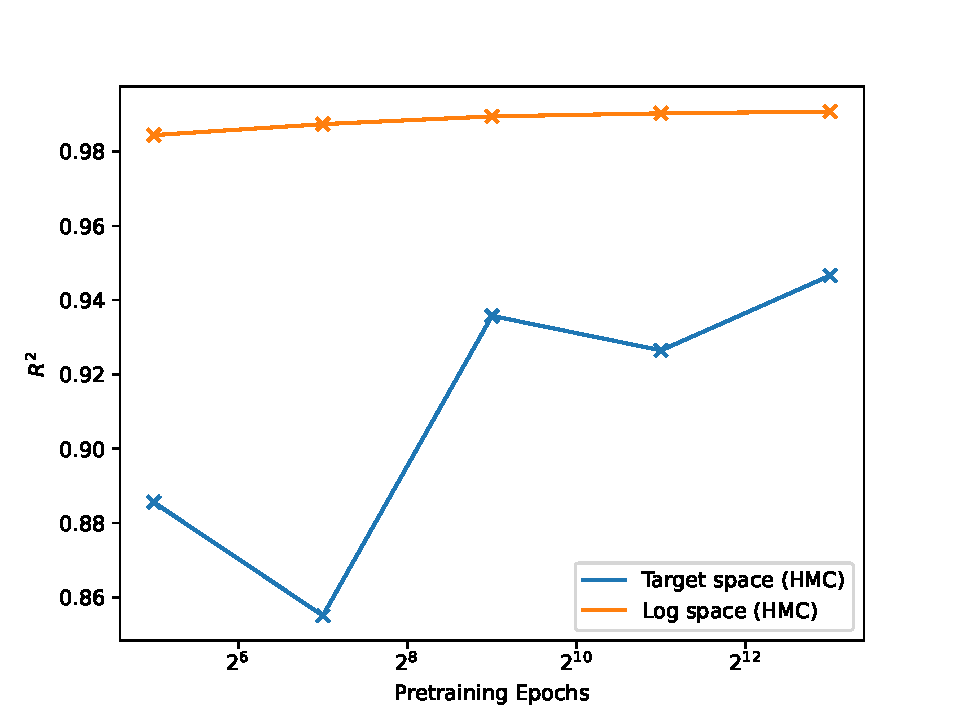
\includegraphics[scale=0.7]{figures/r2_scores/r2_score_vs_pretraining.pdf}
    \caption{The figure shows the computed $R^2$-scores of a model with the architecture 5-20-20-1 with $\tanh(x)$ as the
    hidden activation function. In this case the varying number of the number of epochs run with pretraining starting from 32 all the way up to 8192. The batch size used was 32 with the ADAM optimizer. The number of warm-up steps was 1000 (200 of which were burn-in steps and 800 were adaptation steps). We fixed the Leapfrog steps to $L = 512$ using the HMC sampler. As usual we sampled 1000 neural networks with 10 steps between each sample.
    }
    \label{fig:r2_score_vs_pretraining}
\end{figure}

In figure \ref{fig:std_residual_vs_pretraining}, we
show the computed standardized residuals in log space. The figure demonstrates a pretty noticable improvement as the amount of pretraining increases, up to a point. Once we surpass 2048 epochs of pretraining, we see a slight degradation of the model performance with a larger spread in the residual distribution. But we can rest assured that pretraining can be used to increase the performance of the trained BNN when everything else is held fixed, and should thus be applied as part of the training procedure. Note that the model used here consists of a rather small number of parameters. We performed pretraining of the models on a GPU which yielded less than 10\% GPU utilization, while the MCMC sampling of the model parameters required $\sim 90\%$ GPU utilization. Hence pretraining with models of this size may be better performed on either a built-in GPU on an SoC such as the one shipped with an Apple Silicon SoC. Else, the pretraining should perhaps be employed on a multi-core CPU device.
\begin{figure}[H]
    \centering
    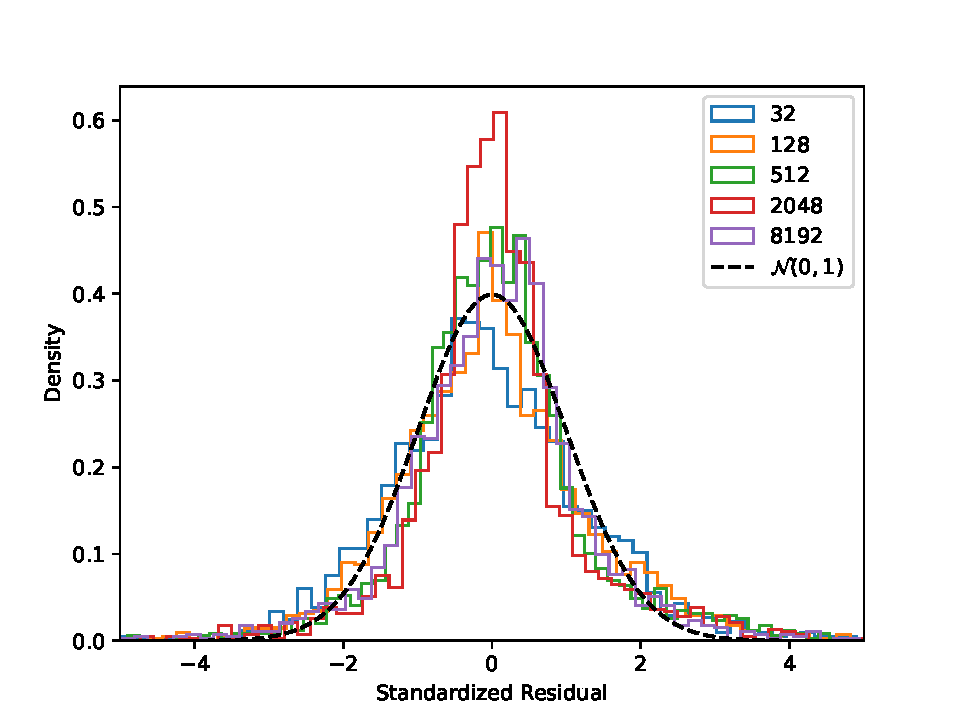
\includegraphics[scale=0.7]{figures/standardized_residuals/effect_of_pretraining/standardized_residuals_hmc_vs_pretraining_steps.pdf}
    \caption{The figure shows the standardized residuals of a model with the architecture 5-20-20-1 with $\tanh(x)$ as the
    hidden activation function. In this case the varying number of the number of epochs run with pretraining starting from 32 all the way up to 8192. The batch size used was 32, the number of warm-up steps was 1000 (200 of which were burn-in steps and 800 were adaptation steps). We fixed the Leapfrog steps to $L = 512$ using the HMC sampler. The ADAM optimizer was used for the pretraining phase. As usual we sampled 1000 neural networks with 10 steps between each sample. The colors indicate the number of pretraining epochs performed. The dotted line is the standard Normal distribution.
    }
    \label{fig:std_residual_vs_pretraining}
\end{figure}

\subsubsection{Effect of Number of Parameters}
Increasing the number of parameters of the BNN model may help capture the underlying process from the data to a larger degree. The typical problems posed by the \textit{bias-variance trade-off} \cite{ml_for_physicists} does not play as significant a role here since the trained model can compute a sample variance along with its prediction. The concept is that increasing the complexity of the model class will increase its ability to capture nuances in the training data which consequentially decreases its ability to generalize well to unseen data. Bayesian neural networks are by no means immune to this effect, however, as the model is still sampled according to the special features found in the training data which in principle may be due to noise or a sample set which does not provide a sufficiently general representation of the underlying process one attempt to capture with the regression model. As explained in section \ref{sec:perf_metrics}, the dataset produced by {\tt Prospino} contains very little noise and thus specializing the model to the inherent noise is not the issue. We did, however, see outliers and asymmetries in figure \ref{fig:dataset_masses} and figure \ref{fig:dataset_mixing_angles}. If a model has a large number of parameters, then, the training may produce a BNN model that generalizes poorly to the unseen test data because it attempts to account for the nuances in the training data. Moreover, the dataset we use is fairly small ($\sim 15000$ datapoints in total), which can exacerbate the effect.

In figure~\ref{fig:r2_scores_vs_num_params} we show the computed $R^2$ score on the training and test data as a function of number of nodes $n$ placed in the hidden layer of models with the architecture 5-$n$-1. The hidden activation used was $\tanh(x)$. The training was carried out with 1000 warm-up steps with the usual division of 20\% burn-in steps and 80\% allocated to adaptation of the step size in the Leapfrog integrator. We performed 2500 pretraining steps with a batch size of 32 for each model. When using the HMC sampler, we fixed the number of Leapfrog steps to $L = 512$. For the NUTS sampler, we allowed a maximum of $L = 4096$ Leapfrog steps. We sampled 1000 networks in each cases, skipping 10 networks between each stored sample. The models trained with the HMC sampler increase in performance up until a maximum after which the performance degrades, which may be explained by the fixed number of Leapfrog steps in an increasingly higher-dimensional parameter space. Moreover, the dataset used is fairly small for $7n + 1$ parameters in total as $n$ increases (which in the highest case of $n = 2^{13} = 8192$ parameters imply 57345 parameters per sampled neural network). 

\begin{figure}[H]
    \centering
    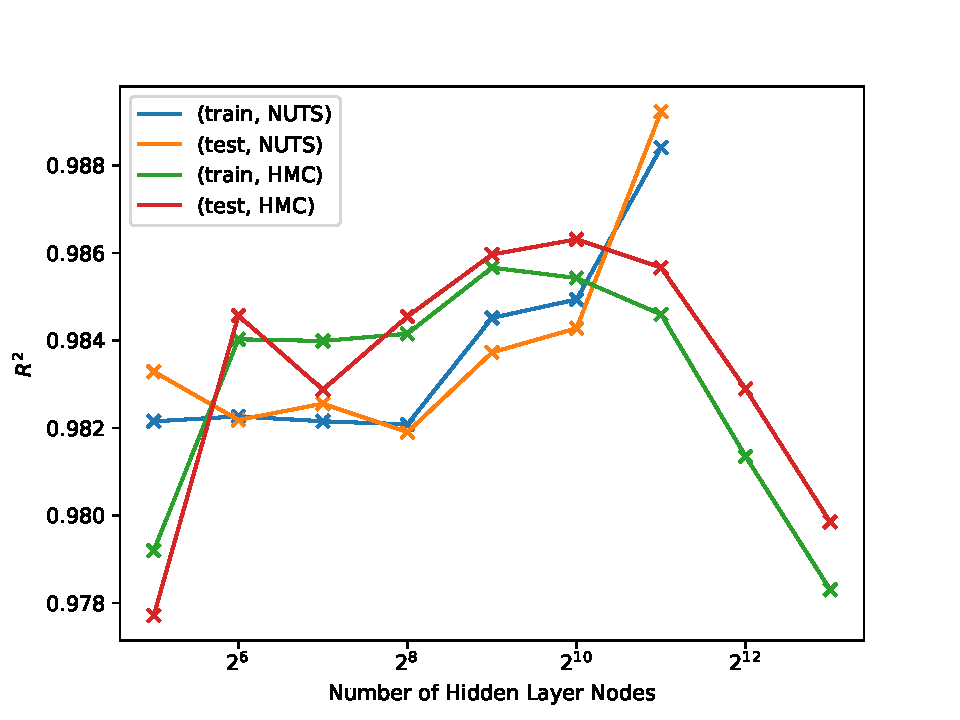
\includegraphics[scale=0.7]{figures/r2_scores/r2_score_vs_num_params_log_space.pdf}
    \caption{
        The figure shows the $R^2$-score computed on the training and test data as a function of number of nodes $n$ in the hidden layer of models with architechture 5-$n$-1, yielding a total of $5n + 1$ parameters. The hidden layer activation used was $\tanh(x)$.
        The models were trained with 1000 warm-up steps (20\% burn-in and 80\% adaptation), gathering 1000 neural networks with 10 steps between each sample. We used 2500 pretraining epochs with a batch size of 32. 
        When using the HMC sampler, we fixed the number of Leapfrog steps to $L = 512$. When using NUTS, we set a maximum of $L = 4096$ Leapfrog steps. 
    }\label{fig:r2_scores_vs_num_params}
\end{figure}



In figure \ref{fig:standardized_residual_vs_params}, we show the computed standardized residual distribution on the test data of the same models, which gives us an idea of the performance the BNNs have on this dataset as a function of the number of parameters. From the figures we can observe that the models trained with $n = 2048$ produced a distribution which lies well inside of the standard Normal distribution albeit with tails extending outwards in both directions about zero. Unfortunately, the data for NUTS beyond this point was not measured due to time constraints. We can note, however, that increasing the parameters beyond a certain point when using HMC seems to appears to degrade the performance which is consistent with the discussion on the bias-variance trade-off we initiated this section with.

\begin{figure}[H]
    \centering
    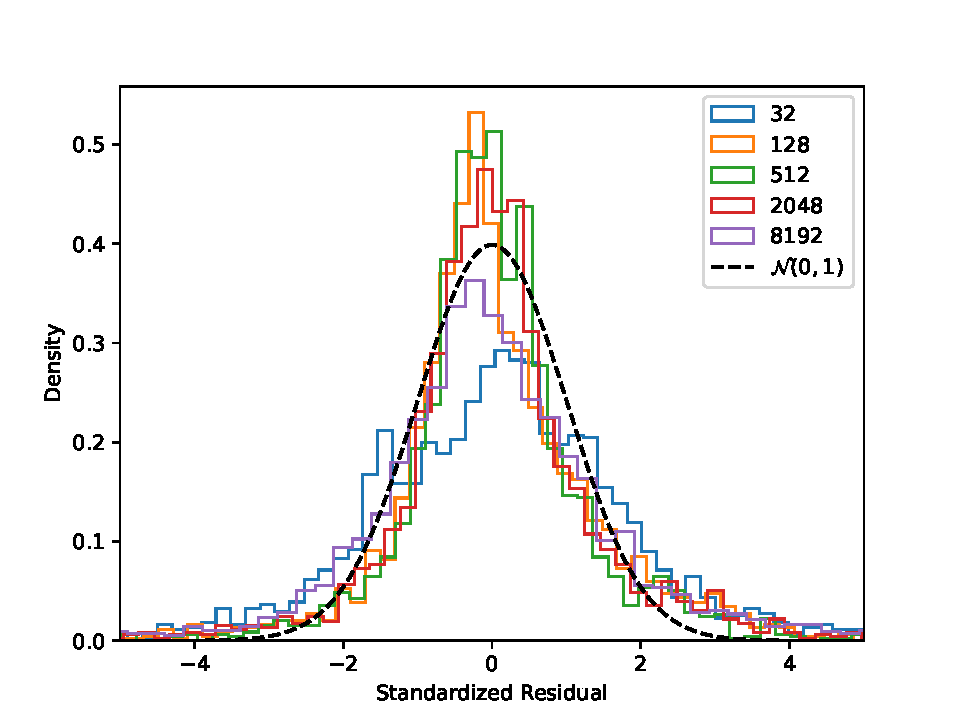
\includegraphics[scale=0.7]{figures/standardized_residuals/effect_of_num_params/standardized_residual_HMC.pdf}
    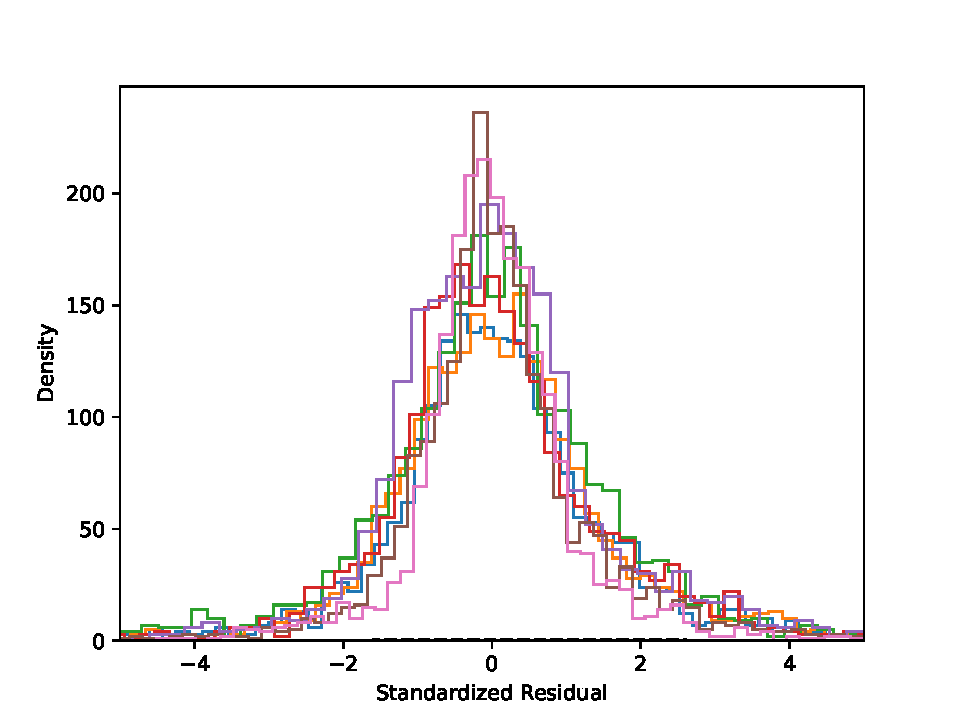
\includegraphics[scale=0.7]{figures/standardized_residuals/effect_of_num_params/standardized_residual_NUTS.pdf}
    \caption{
        The figure shows the standardized residuals of models with an architecture 5-$n$-1 with $\tanh(x)$ as the hidden layer activation. The models were trained with 1000 warm-up steps (20\% burn-in and 80\% adaptation), drawing 1000 neural networks with 10 steps between each drawn sample. We used 2500 pretraining epochs with a batch size of 32 using the ADAM optimizer. The figure on top shows results of models trained with the HMC sampler where we fixed the number of Leapfrog steps to $L = 512$. The figure on the bottom shows the results of models trained with NUTS using a maximum of $L = 4096$ Leapfrog steps. The black dotted line shows the standard Normal distribution drawn in.
    }
    \label{fig:standardized_residual_vs_params}
\end{figure}

\subsection{Predictive Distributions}
As we discussed in chapter \ref{chap:bayesian_ml}, one of the primary objects we seek to compute
in Bayesian ML is the predictive distribution $p(y^*|x^*, D)$ for a target $y^*$ given an unseen input point $x^*$ and
a training dataset $D$. Thus far, we have not explicitly explored the predictive distributions the BNN models compute but instead focused the effects it has using certain metrics. Using BNNs as a substitute for direct calculations of NLO predictions can be a dangerous decision if care is not taken to understand the probabilistic nature of the model class. We shall thus turn our attention to exploring the predictive distribution in this section.

In figure \ref{fig:predictive_distributions}, we show the predictive distribution computed with model 3 in table \ref{tab:deep_models}. In the figure on top, the sample mean approximates the true target well with a fairly small spread in the distribution which is a desirable outcome in most cases. There are, however, ill performing cases as well which we demonstrate in the figure at the bottom. Here the true target lies entirely outside the predictive distribution. Thus care must be taken to understand when a BNNs prediction is reliable and when it is not. 
\begin{figure}[H]
    \centering
    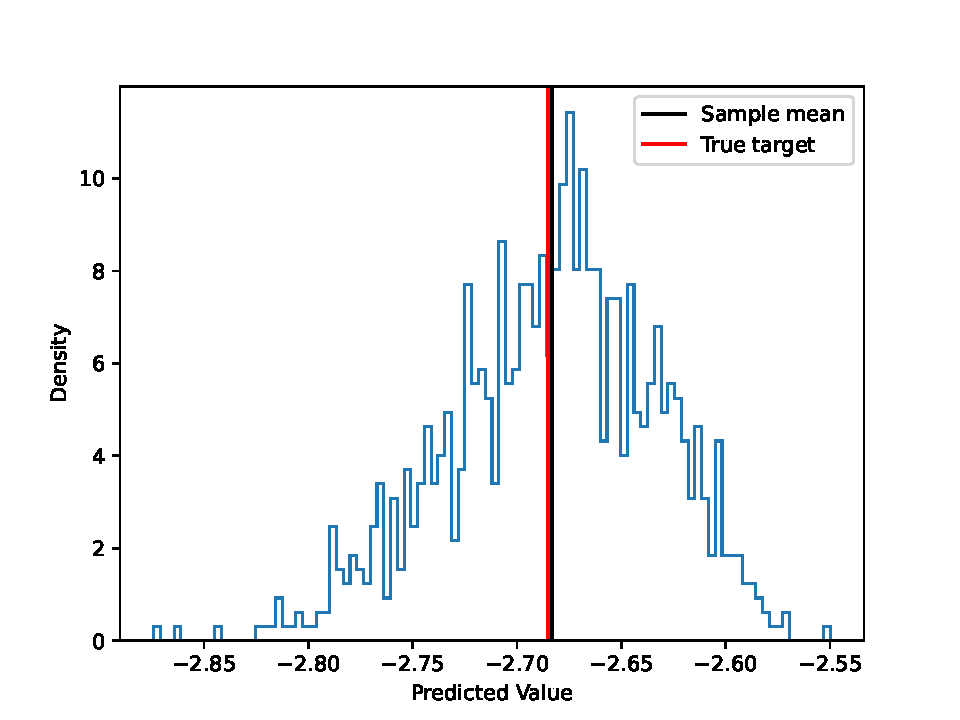
\includegraphics[scale=0.5]{figures/predictive_distributions/predictive_distribution_point_idx_360.pdf}
    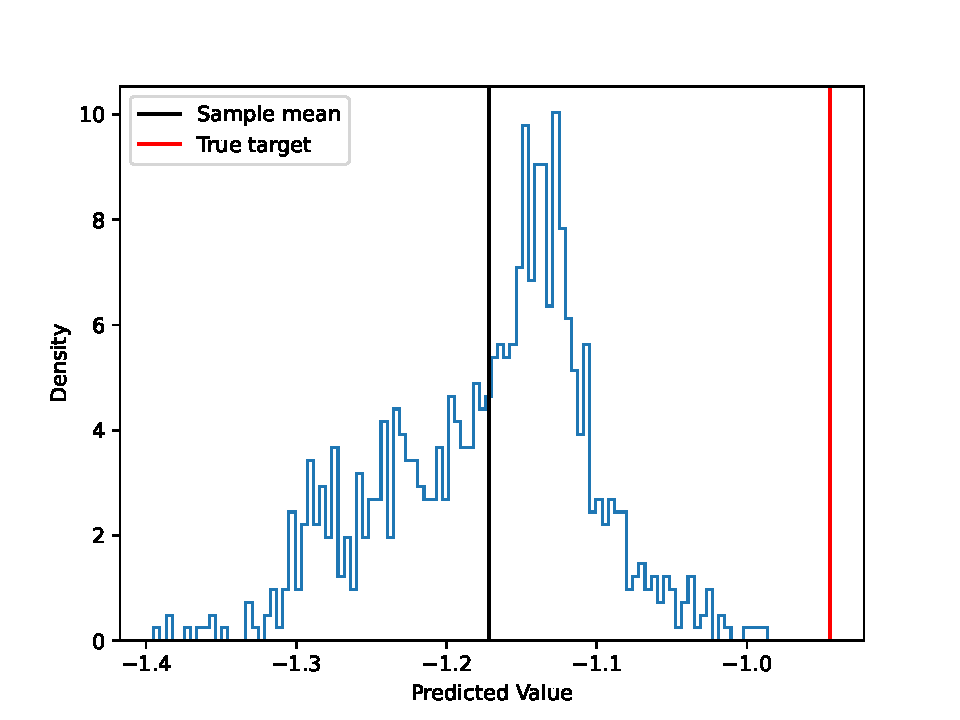
\includegraphics[scale=0.5]{figures/predictive_distributions/predictive_distribution_point_idx_2052.pdf}
    \caption{
        The figure shows the predictive distribution estimated by use of model 3 in table \ref{tab:deep_models} for two randomly chosen points from the test set. The red line shows the true target and the black line shows the predicted sample mean obtained from the distribution. The figure on top demonstrates a case where the sample mean is approximately the same as the target, while the figure at the bottom demonstrates a case where the true target lies entirely outside the predictive distrbution. 
    }
    \label{fig:predictive_distributions}
\end{figure}


We can deal with this problem by empirically counting how many targets $y \in [\mu - k\sigma, \mu + k \sigma]$ for $k = 1, 2, 3, 4, 5$ where $\mu$ represents the sample mean and $\sigma^2$ represents the sample variance of each predictive distribution computed by the BNN model. In principle there is no need for $k$ to be an integer, and a finite grid of points $k \in (0, \infty)$ can be used instead such that an arbitrary desired accuracy can be specified. 
For comparative purposes, note that for $k = 1, 2, 3$ the expected percentages of points should be approximately 68\%, 96\% and 99.7\% for a Gaussian distribution, respectively. Though, we have no \textit{a priori} reason to assume the preditive distributions are Gaussian, the percentages serve as useful reference values.

We illustrate the results of this analysis in figure \ref{fig:confidence} performed on the training, validation and test data. Clearly there exists a small percentage of ill cases where the target lies far away from the predicted mean. The result does at least tell us that more than 95\% of the targets lie within $\mu \pm 3\sigma$ in their respective predictive distribution. This is however lower than the expected value of 96\% within $\mu \pm 2\sigma$.
\begin{figure}[H]
    \centering
    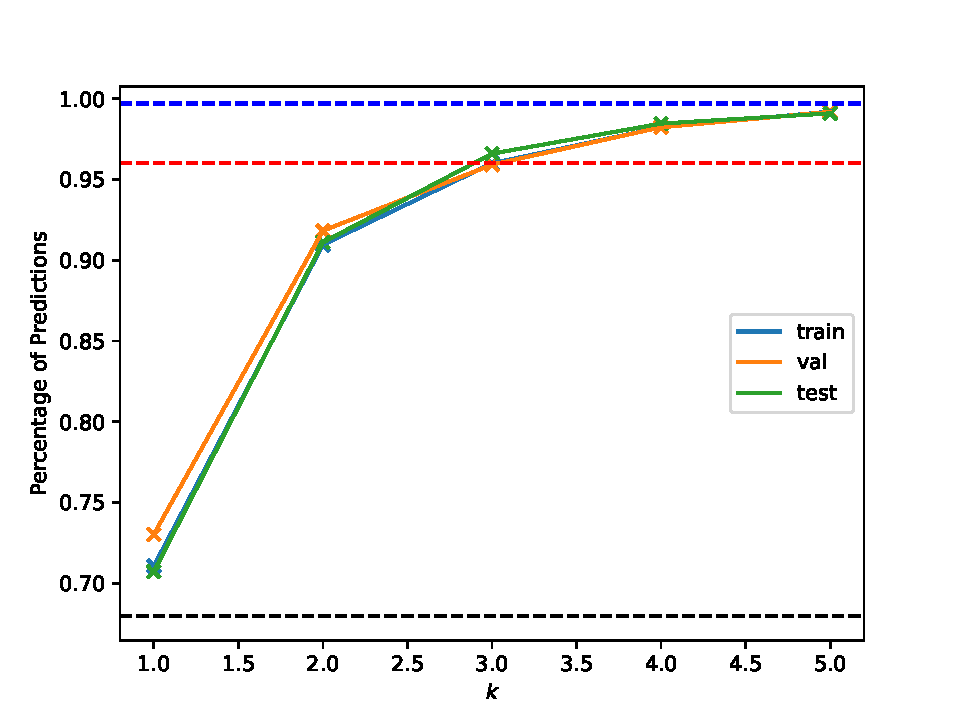
\includegraphics[scale=0.7]{figures/confidence_estimation/good_vs_bad_cases_confidence.pdf}
    \caption{
        The figure shows the predictive distribution estimated by use of model 3 in table \ref{tab:deep_models}
        computed on all datapoints in the training, validation and test data. The black line shows the 95\% line. The crosses indicate measured data with training data shown in blue, validation data shown in orange and test data shown in green. The $y$-axis shows the percentage of all targets lie on the interval $[\mu - k\sigma, \mu + k\sigma]$ for $k=1,2,3,4,5$ where $\mu$ is the sample mean and $\sigma^2$ is the sample variance of the predictive distribution.
    }
    \label{fig:confidence}
\end{figure}






